\documentclass[oneside,a4paper]{report}
\usepackage{color}
\usepackage{longtable}
\usepackage{titlesec}
\usepackage[hidelinks]{hyperref}
\usepackage{ulem}
\usepackage{graphicx}
\usepackage{fancyhdr}
\usepackage[T1]{fontenc}
\usepackage[headheight=25pt,margin=0.7in,top=1.5in,bottom=1in,right=1in,left=1in]{geometry}

\hypersetup{colorlinks=true,linktoc=none,citecolor=black,urlcolor=blue}
\hypersetup{linktocpage=false,linkcolor=black}

\pagestyle{fancy}
\fancyhead[R]{
\includegraphics[width=2cm]{./latex/resources/kitlogo.png}}
\fancyhead[L]{\leftmark}

\fancypagestyle{plain}{
        \rhead{
\includegraphics[width=2cm]{./latex/resources/kitlogo.png}}
        \lhead{\leftmark}
}


\renewcommand{\arraystretch}{2}

\titleformat{\chapter}[hang]
 {\normalfont\bfseries\LARGE}{\thechapter. }{0pt}{\LARGE}
\titleformat{\section}[hang]
 {\normalfont\bfseries\Large}{\thesection. }{0pt}{\Large}
\titleformat{\paragraph}[hang]
 {\normalfont\bfseries\normalsize}{}{}{}

\titlespacing*{\chapter}{0pt}{-20pt}{10pt}

\begin{document}
  \begin{titlepage}
	\centering
	{\scshape\LARGE Karlsruhe Institute of Technology \par}
	\vspace{1cm}
	{\scshape\Large Software Engineering Practice\par}
	\vspace{0.5cm}
	{\scshape\Large WINTER TERM 2015/2016\par}
	\vspace{1.5cm}
	{\Huge\bfseries rootJS - module guide\par}
	\vspace{0.25cm}
	{\Large\bfseries Node.js bindings for ROOT 6\par}
	\vspace{2cm}
	{\Large\itshape Jonas Schwabe\par}
	{\Large\itshape Theo Beffart\par}
	{\Large\itshape Sachin Rajgopal\par}
	{\Large\itshape Christoph Wolff\par}
	{\Large\itshape Christoph Haas\par}

	{\Large\itshape Maximilian Fr\"uh\par}
	\vfill
	supervised by\par
	Dr.~Marek \textsc{Szuba}

	\vfill

	% Bottom of the page
	{\large \date{99.99.9999}\par}
\end{titlepage}

  \tableofcontents
  \clearpage
  %\input{./latex/purpose.tex}
   \chapter{NodeApplication}
describe class NodeApplication here
\section{ctorCallback}
\begin{longtable}{p{3cm} @{\hskip 1cm} p{12cm}}
 \hline
\textit{Name} & \texttt{NodeApplication::ctorCallback(args: FunctionCallbackInfo<Value>)}\\
\hline
 \textit{Visibility} & Public \\
\hline
\textit{Parameters} & \textit{args: FunctionCallbackInfo<Value>}\\
\hline
\textit{Return value} & \textbf{none}\\
  \hline
 \textit{behavior} & describe beahviour \\
\hline
\end{longtable} \pagebreak
 \section{staticCtorCallback}
\begin{longtable}{p{3cm} @{\hskip 1cm} p{12cm}}
 \hline
\textit{Name} & \texttt{NodeApplication::staticCtorCallback(args: FunctionCallbackInfo<Value>)}\\
\hline
 \textit{Visibility} & Public \\
\hline
\textit{Parameters} & \textit{args: FunctionCallbackInfo<Value>}\\
\hline
\textit{Return value} & \textbf{none}\\
  \hline
 \textit{behavior} & describe beahviour \\
\hline
\end{longtable} \pagebreak
 \section{memberGetterCallback}
\begin{longtable}{p{3cm} @{\hskip 1cm} p{12cm}}
 \hline
\textit{Name} & \texttt{NodeApplication::memberGetterCallback(property: Local<String>, info: PropertyCallbackInfo<Value>)}\\
\hline
 \textit{Visibility} & Public \\
\hline
\textit{Parameters} & \textit{property: Local<String>, info: PropertyCallbackInfo<Value>}\\
\hline
\textit{Return value} & \textbf{none}\\
  \hline
 \textit{behavior} & describe beahviour \\
\hline
\end{longtable} \pagebreak
 \section{memberSetterCallback}
\begin{longtable}{p{3cm} @{\hskip 1cm} p{12cm}}
 \hline
\textit{Name} & \texttt{NodeApplication::memberSetterCallback(property: Local<String>, value: Local<Value>, info: PropertyCallbackInfo<Value>)}\\
\hline
 \textit{Visibility} & Public \\
\hline
\textit{Parameters} & \textit{property: Local<String>, value: Local<Value>, info: PropertyCallbackInfo<Value>}\\
\hline
\textit{Return value} & \textbf{none}\\
  \hline
 \textit{behavior} & describe beahviour \\
\hline
\end{longtable} \pagebreak
 \section{memberFunctionCallback}
\begin{longtable}{p{3cm} @{\hskip 1cm} p{12cm}}
 \hline
\textit{Name} & \texttt{NodeApplication::memberFunctionCallback(args: FunctionCallbackInfo<Value>)}\\
\hline
 \textit{Visibility} & Public \\
\hline
\textit{Parameters} & \textit{args: FunctionCallbackInfo<Value>}\\
\hline
\textit{Return value} & \textbf{none}\\
  \hline
 \textit{behavior} & describe beahviour \\
\hline
\end{longtable} \pagebreak
 \section{staticGetterCallback}
\begin{longtable}{p{3cm} @{\hskip 1cm} p{12cm}}
 \hline
\textit{Name} & \texttt{NodeApplication::staticGetterCallback(property: Local<String>, info: PropertyCallbackInfo<Value>)}\\
\hline
 \textit{Visibility} & Public \\
\hline
\textit{Parameters} & \textit{property: Local<String>, info: PropertyCallbackInfo<Value>}\\
\hline
\textit{Return value} & \textbf{none}\\
  \hline
 \textit{behavior} & describe beahviour \\
\hline
\end{longtable} \pagebreak
 \section{staticSetterCallback}
\begin{longtable}{p{3cm} @{\hskip 1cm} p{12cm}}
 \hline
\textit{Name} & \texttt{NodeApplication::staticSetterCallback(property: Local<String>, value: Local<Value>, info: PropertyCallbackInfo<Value>)}\\
\hline
 \textit{Visibility} & Public \\
\hline
\textit{Parameters} & \textit{property: Local<String>, value: Local<Value>, info: PropertyCallbackInfo<Value>}\\
\hline
\textit{Return value} & \textbf{none}\\
  \hline
 \textit{behavior} & describe beahviour \\
\hline
\end{longtable} \pagebreak
 \section{staticFunctionCallback}
\begin{longtable}{p{3cm} @{\hskip 1cm} p{12cm}}
 \hline
\textit{Name} & \texttt{NodeApplication::staticFunctionCallback(args: FunctionCallbackInfo<Value>)}\\
\hline
 \textit{Visibility} & Public \\
\hline
\textit{Parameters} & \textit{args: FunctionCallbackInfo<Value>}\\
\hline
\textit{Return value} & \textbf{none}\\
  \hline
 \textit{behavior} & describe beahviour \\
\hline
\end{longtable} \pagebreak
 \section{Initialize}
\begin{longtable}{p{3cm} @{\hskip 1cm} p{12cm}}
 \hline
\textit{Name} & \texttt{NodeApplication::Initialize(exports: Local<Object>, module: Local<Object>)}\\
\hline
 \textit{Visibility} & Public \\
\hline
\textit{Parameters} & \textit{exports: Local<Object>, module: Local<Object>}\\
\hline
\textit{Return value} & \textbf{none}\\
  \hline
 \textit{behavior} & describe beahviour \\
\hline
\end{longtable} \pagebreak
 \section{Instance}
\begin{longtable}{p{3cm} @{\hskip 1cm} p{12cm}}
 \hline
\textit{Name} & \texttt{NodeApplication::Instance()}\\
\hline
 \textit{Visibility} & Public \\
\hline
\textit{Parameters} & \textit{none}\\
\hline
\textit{Return value} & \textbf{ NodeApplication} describe return value\\
  \hline
 \textit{behavior} & describe beahviour \\
\hline
\end{longtable} \pagebreak
 \section{getIsolate}
\begin{longtable}{p{3cm} @{\hskip 1cm} p{12cm}}
 \hline
\textit{Name} & \texttt{NodeApplication::getIsolate()}\\
\hline
 \textit{Visibility} & Public \\
\hline
\textit{Parameters} & \textit{none}\\
\hline
\textit{Return value} & \textbf{ Isolate*} describe return value\\
  \hline
 \textit{behavior} & describe beahviour \\
\hline
\end{longtable} \pagebreak
 \section{getExports}
\begin{longtable}{p{3cm} @{\hskip 1cm} p{12cm}}
 \hline
\textit{Name} & \texttt{NodeApplication::getExports()}\\
\hline
 \textit{Visibility} & Public \\
\hline
\textit{Parameters} & \textit{none}\\
\hline
\textit{Return value} & \textbf{ Local<Object>} describe return value\\
  \hline
 \textit{behavior} & describe beahviour \\
\hline
\end{longtable} \pagebreak
 \section{getTemplateFactory}
\begin{longtable}{p{3cm} @{\hskip 1cm} p{12cm}}
 \hline
\textit{Name} & \texttt{NodeApplication::getTemplateFactory()}\\
\hline
 \textit{Visibility} & Public \\
\hline
\textit{Parameters} & \textit{none}\\
\hline
\textit{Return value} & \textbf{ TemplateFactory} describe return value\\
  \hline
 \textit{behavior} & describe beahviour \\
\hline
\end{longtable} \pagebreak
 \section{getFunctionFactory}
\begin{longtable}{p{3cm} @{\hskip 1cm} p{12cm}}
 \hline
\textit{Name} & \texttt{NodeApplication::getFunctionFactory()}\\
\hline
 \textit{Visibility} & Public \\
\hline
\textit{Parameters} & \textit{none}\\
\hline
\textit{Return value} & \textbf{ ProxyFunctionFactory} describe return value\\
  \hline
 \textit{behavior} & describe beahviour \\
\hline
\end{longtable} \pagebreak
 \section{getObjectFactory}
\begin{longtable}{p{3cm} @{\hskip 1cm} p{12cm}}
 \hline
\textit{Name} & \texttt{NodeApplication::getObjectFactory()}\\
\hline
 \textit{Visibility} & Public \\
\hline
\textit{Parameters} & \textit{none}\\
\hline
\textit{Return value} & \textbf{ ProxyObjectFactory} describe return value\\
  \hline
 \textit{behavior} & describe beahviour \\
\hline
\end{longtable} \pagebreak
 \chapter{TemplateFactory}
describe class TemplateFactory here
\section{createTemplate}
\begin{longtable}{p{3cm} @{\hskip 1cm} p{12cm}}
 \hline
\textit{Name} & \texttt{TemplateFactory::createTemplate(clazz: TClassRef)}\\
\hline
 \textit{Visibility} & Public \\
\hline
\textit{Parameters} & \textit{clazz: TClassRef}\\
\hline
\textit{Return value} & \textbf{ Local<FunctionTemplate>} describe return value\\
  \hline
 \textit{behavior} & describe beahviour \\
\hline
\end{longtable} \pagebreak
 \chapter{TemplateCache}
describe class TemplateCache here
\section{contains}
\begin{longtable}{p{3cm} @{\hskip 1cm} p{12cm}}
 \hline
\textit{Name} & \texttt{TemplateCache::contains(type: TClassRef)}\\
\hline
 \textit{Visibility} & Public \\
\hline
\textit{Parameters} & \textit{type: TClassRef}\\
\hline
\textit{Return value} & \textbf{ bool} describe return value\\
  \hline
 \textit{behavior} & describe beahviour \\
\hline
\end{longtable} \pagebreak
 \section{get}
\begin{longtable}{p{3cm} @{\hskip 1cm} p{12cm}}
 \hline
\textit{Name} & \texttt{TemplateCache::get(type: TClassRef)}\\
\hline
 \textit{Visibility} & Public \\
\hline
\textit{Parameters} & \textit{type: TClassRef}\\
\hline
\textit{Return value} & \textbf{ Local<FunctionTemplate>} describe return value\\
  \hline
 \textit{behavior} & describe beahviour \\
\hline
\end{longtable} \pagebreak
 \section{store}
\begin{longtable}{p{3cm} @{\hskip 1cm} p{12cm}}
 \hline
\textit{Name} & \texttt{TemplateCache::store(type: TClassRef, tpl: Local<FunctionTemplate>)}\\
\hline
 \textit{Visibility} & Public \\
\hline
\textit{Parameters} & \textit{type: TClassRef, tpl: Local<FunctionTemplate>}\\
\hline
\textit{Return value} & \textbf{none}\\
  \hline
 \textit{behavior} & describe beahviour \\
\hline
\end{longtable} \pagebreak
 \chapter{ProxyFunctionFactory}
describe class ProxyFunctionFactory here
\section{createProxyFunction}
\begin{longtable}{p{3cm} @{\hskip 1cm} p{12cm}}
 \hline
\textit{Name} & \texttt{ProxyFunctionFactory::createProxyFunction(info: TMethod)}\\
\hline
 \textit{Visibility} & Public \\
\hline
\textit{Parameters} & \textit{info: TMethod}\\
\hline
\textit{Return value} & \textbf{ ProxyFunciton} describe return value\\
  \hline
 \textit{behavior} & describe beahviour \\
\hline
\end{longtable} \pagebreak
 \section{fromArgs}
\begin{longtable}{p{3cm} @{\hskip 1cm} p{12cm}}
 \hline
\textit{Name} & \texttt{ProxyFunctionFactory::fromArgs(name: string, clazz: TClassRef, args: FunctionCallbackInfo)}\\
\hline
 \textit{Visibility} & Public \\
\hline
\textit{Parameters} & \textit{name: string, clazz: TClassRef, args: FunctionCallbackInfo}\\
\hline
\textit{Return value} & \textbf{ ProxyFunction} describe return value\\
  \hline
 \textit{behavior} & describe beahviour \\
\hline
\end{longtable} \pagebreak
 \chapter{ProxyFunction}
describe class ProxyFunction here
\section{ProxyFunction}
\begin{longtable}{p{3cm} @{\hskip 1cm} p{12cm}}
 \hline
\textit{Name} & \texttt{ProxyFunction::ProxyFunction(address: void*, info: TFunction)}\\
\hline
 \textit{Visibility} & Public \\
\hline
\textit{Parameters} & \textit{address: void*, info: TFunction}\\
\hline
\textit{Return value} & \textbf{ <<constructor>>} describe return value\\
  \hline
 \textit{behavior} & describe beahviour \\
\hline
\end{longtable} \pagebreak
 \section{convertArgs}
\begin{longtable}{p{3cm} @{\hskip 1cm} p{12cm}}
 \hline
\textit{Name} & \texttt{ProxyFunction::convertArgs(args: FunctionCallbackInfo)}\\
\hline
 \textit{Visibility} & Public \\
\hline
\textit{Parameters} & \textit{args: FunctionCallbackInfo}\\
\hline
\textit{Return value} & \textbf{ ProxyObject[]} describe return value\\
  \hline
 \textit{behavior} & describe beahviour \\
\hline
\end{longtable} \pagebreak
 \section{call}
\begin{longtable}{p{3cm} @{\hskip 1cm} p{12cm}}
 \hline
\textit{Name} & \texttt{ProxyFunction::call(args: ProxyObject[])}\\
\hline
 \textit{Visibility} & Public \\
\hline
\textit{Parameters} & \textit{args: ProxyObject[]}\\
\hline
\textit{Return value} & \textbf{ ProxyObject} describe return value\\
  \hline
 \textit{behavior} & describe beahviour \\
\hline
\end{longtable} \pagebreak
 \section{isTemplateFunction}
\begin{longtable}{p{3cm} @{\hskip 1cm} p{12cm}}
 \hline
\textit{Name} & \texttt{ProxyFunction::isTemplateFunction()}\\
\hline
 \textit{Visibility} & Public \\
\hline
\textit{Parameters} & \textit{none}\\
\hline
\textit{Return value} & \textbf{ bool} describe return value\\
  \hline
 \textit{behavior} & describe beahviour \\
\hline
\end{longtable} \pagebreak
 \chapter{ProxyObjectFactory}
describe class ProxyObjectFactory here
\section{createProxyObject}
\begin{longtable}{p{3cm} @{\hskip 1cm} p{12cm}}
 \hline
\textit{Name} & \texttt{ProxyObjectFactory::createProxyObject(type: TDataMember, holder: ProxyObject)}\\
\hline
 \textit{Visibility} & Public \\
\hline
\textit{Parameters} & \textit{type: TDataMember, holder: ProxyObject}\\
\hline
\textit{Return value} & \textbf{ ProxyObject} describe return value\\
  \hline
 \textit{behavior} & describe beahviour \\
\hline
\end{longtable} \pagebreak
 \chapter{ProxyObject}
describe class ProxyObject here
\section{ProxyObject}
\begin{longtable}{p{3cm} @{\hskip 1cm} p{12cm}}
 \hline
\textit{Name} & \texttt{ProxyObject::ProxyObject(address: void*, type: TDataMember)}\\
\hline
 \textit{Visibility} & Public \\
\hline
\textit{Parameters} & \textit{address: void*, type: TDataMember}\\
\hline
\textit{Return value} & \textbf{ <<constructor>>} describe return value\\
  \hline
 \textit{behavior} & describe beahviour \\
\hline
\end{longtable} \pagebreak
 \section{getAddress}
\begin{longtable}{p{3cm} @{\hskip 1cm} p{12cm}}
 \hline
\textit{Name} & \texttt{ProxyObject::getAddress()}\\
\hline
 \textit{Visibility} & Public \\
\hline
\textit{Parameters} & \textit{none}\\
\hline
\textit{Return value} & \textbf{ void*} describe return value\\
  \hline
 \textit{behavior} & describe beahviour \\
\hline
\end{longtable} \pagebreak
 \section{getType}
\begin{longtable}{p{3cm} @{\hskip 1cm} p{12cm}}
 \hline
\textit{Name} & \texttt{ProxyObject::getType()}\\
\hline
 \textit{Visibility} & Public \\
\hline
\textit{Parameters} & \textit{none}\\
\hline
\textit{Return value} & \textbf{ TDataMember} describe return value\\
  \hline
 \textit{behavior} & describe beahviour \\
\hline
\end{longtable} \pagebreak
 \section{set}
\begin{longtable}{p{3cm} @{\hskip 1cm} p{12cm}}
 \hline
\textit{Name} & \texttt{ProxyObject::set(value: ProxyObject)}\\
\hline
 \textit{Visibility} & Public \\
\hline
\textit{Parameters} & \textit{value: ProxyObject}\\
\hline
\textit{Return value} & \textbf{none}\\
  \hline
 \textit{behavior} & describe beahviour \\
\hline
\end{longtable} \pagebreak
 \section{get}
\begin{longtable}{p{3cm} @{\hskip 1cm} p{12cm}}
 \hline
\textit{Name} & \texttt{ProxyObject::get()}\\
\hline
 \textit{Visibility} & Public \\
\hline
\textit{Parameters} & \textit{none}\\
\hline
\textit{Return value} & \textbf{ Local<Value>} describe return value\\
  \hline
 \textit{behavior} & describe beahviour \\
\hline
\end{longtable} \pagebreak
 \section{isPrimitive}
\begin{longtable}{p{3cm} @{\hskip 1cm} p{12cm}}
 \hline
\textit{Name} & \texttt{ProxyObject::isPrimitive()}\\
\hline
 \textit{Visibility} & Public \\
\hline
\textit{Parameters} & \textit{none}\\
\hline
\textit{Return value} & \textbf{ bool} describe return value\\
  \hline
 \textit{behavior} & describe beahviour \\
\hline
\end{longtable} \pagebreak

   \chapter{ClassHelper}
describe class ClassHelper here
\section{IsNamespace}
\begin{longtable}{p{3cm} @{\hskip 1cm} p{12cm}}
\hline
\textit{Name} & \texttt{ClassHelper::IsNamespace(scope: TCppScope_t)}\\
\hline
\textit{Visibility} & \\
\hline
\textit{Parameters} & \textit{scope: TCppScope_t}\\
\hline
\textit{Return value} & \textbf{ Bool_t} describe return value\\
 \hline
\textit{behavior} & describe beahviour \\
\hline
\end{longtable} \pagebreak
\section{IsAbstract}
\begin{longtable}{p{3cm} @{\hskip 1cm} p{12cm}}
\hline
\textit{Name} & \texttt{ClassHelper::IsAbstract(klass: TCppType_t)}\\
\hline
\textit{Visibility} & \\
\hline
\textit{Parameters} & \textit{klass: TCppType_t}\\
\hline
\textit{Return value} & \textbf{ Bool_t} describe return value\\
 \hline
\textit{behavior} & describe beahviour \\
\hline
\end{longtable} \pagebreak
\section{IsEnum}
\begin{longtable}{p{3cm} @{\hskip 1cm} p{12cm}}
\hline
\textit{Name} & \texttt{ClassHelper::IsEnum(type_name: conSTstd::string&)}\\
\hline
\textit{Visibility} & \\
\hline
\textit{Parameters} & \textit{type_name: conSTstd::string&}\\
\hline
\textit{Return value} & \textbf{ Bool_t} describe return value\\
 \hline
\textit{behavior} & describe beahviour \\
\hline
\end{longtable} \pagebreak
\section{IsStruct}
\begin{longtable}{p{3cm} @{\hskip 1cm} p{12cm}}
\hline
\textit{Name} & \texttt{ClassHelper::IsStruct(type_name: conSTstd::string&)}\\
\hline
\textit{Visibility} & \\
\hline
\textit{Parameters} & \textit{type_name: conSTstd::string&}\\
\hline
\textit{Return value} & \textbf{ Bool_t} describe return value\\
 \hline
\textit{behavior} & describe beahviour \\
\hline
\end{longtable} \pagebreak
\section{GetFinalName}
\begin{longtable}{p{3cm} @{\hskip 1cm} p{12cm}}
\hline
\textit{Name} & \texttt{ClassHelper::GetFinalName(klass: TCppType_t)}\\
\hline
\textit{Visibility} & \\
\hline
\textit{Parameters} & \textit{klass: TCppType_t}\\
\hline
\textit{Return value} & \textbf{ stdstring} describe return value\\
 \hline
\textit{behavior} & describe beahviour \\
\hline
\end{longtable} \pagebreak
\section{GetScopedFinalName}
\begin{longtable}{p{3cm} @{\hskip 1cm} p{12cm}}
\hline
\textit{Name} & \texttt{ClassHelper::GetScopedFinalName(klass: TCppType_t)}\\
\hline
\textit{Visibility} & \\
\hline
\textit{Parameters} & \textit{klass: TCppType_t}\\
\hline
\textit{Return value} & \textbf{ stdstring} describe return value\\
 \hline
\textit{behavior} & describe beahviour \\
\hline
\end{longtable} \pagebreak
\section{GetNumBases}
\begin{longtable}{p{3cm} @{\hskip 1cm} p{12cm}}
\hline
\textit{Name} & \texttt{ClassHelper::GetNumBases(klass: TCppType_t)}\\
\hline
\textit{Visibility} & \\
\hline
\textit{Parameters} & \textit{klass: TCppType_t}\\
\hline
\textit{Return value} & \textbf{ TCppIndex_t} describe return value\\
 \hline
\textit{behavior} & describe beahviour \\
\hline
\end{longtable} \pagebreak
\section{GetBaseName}
\begin{longtable}{p{3cm} @{\hskip 1cm} p{12cm}}
\hline
\textit{Name} & \texttt{ClassHelper::GetBaseName(klass: TCppType_t, ibase: TCppIndex_t)}\\
\hline
\textit{Visibility} & \\
\hline
\textit{Parameters} & \textit{klass: TCppType_t, ibase: TCppIndex_t}\\
\hline
\textit{Return value} & \textbf{ stdstring} describe return value\\
 \hline
\textit{behavior} & describe beahviour \\
\hline
\end{longtable} \pagebreak
\section{IsSubtype}
\begin{longtable}{p{3cm} @{\hskip 1cm} p{12cm}}
\hline
\textit{Name} & \texttt{ClassHelper::IsSubtype(derived: TCppType_t, base: TCppType_t)}\\
\hline
\textit{Visibility} & \\
\hline
\textit{Parameters} & \textit{derived: TCppType_t, base: TCppType_t}\\
\hline
\textit{Return value} & \textbf{ Bool_t} describe return value\\
 \hline
\textit{behavior} & describe beahviour \\
\hline
\end{longtable} \pagebreak
\section{GetNumDatamembers}
\begin{longtable}{p{3cm} @{\hskip 1cm} p{12cm}}
\hline
\textit{Name} & \texttt{ClassHelper::GetNumDatamembers(scope: TCppScope_t)}\\
\hline
\textit{Visibility} & \\
\hline
\textit{Parameters} & \textit{scope: TCppScope_t}\\
\hline
\textit{Return value} & \textbf{ TCppIndex_t} describe return value\\
 \hline
\textit{behavior} & describe beahviour \\
\hline
\end{longtable} \pagebreak
\section{GetDatamemberName}
\begin{longtable}{p{3cm} @{\hskip 1cm} p{12cm}}
\hline
\textit{Name} & \texttt{ClassHelper::GetDatamemberName(scope: TCppScope_t, idata: TCppIndex_t)}\\
\hline
\textit{Visibility} & \\
\hline
\textit{Parameters} & \textit{scope: TCppScope_t, idata: TCppIndex_t}\\
\hline
\textit{Return value} & \textbf{ stdstring} describe return value\\
 \hline
\textit{behavior} & describe beahviour \\
\hline
\end{longtable} \pagebreak
\section{GetDatamemberType}
\begin{longtable}{p{3cm} @{\hskip 1cm} p{12cm}}
\hline
\textit{Name} & \texttt{ClassHelper::GetDatamemberType(scope: TCppScope_t, idata: TCppIndex_t)}\\
\hline
\textit{Visibility} & \\
\hline
\textit{Parameters} & \textit{scope: TCppScope_t, idata: TCppIndex_t}\\
\hline
\textit{Return value} & \textbf{ stdstring} describe return value\\
 \hline
\textit{behavior} & describe beahviour \\
\hline
\end{longtable} \pagebreak
\section{GetDatamemberOffset}
\begin{longtable}{p{3cm} @{\hskip 1cm} p{12cm}}
\hline
\textit{Name} & \texttt{ClassHelper::GetDatamemberOffset(scope: TCppScope_t, idata: TCppIndex_t)}\\
\hline
\textit{Visibility} & \\
\hline
\textit{Parameters} & \textit{scope: TCppScope_t, idata: TCppIndex_t}\\
\hline
\textit{Return value} & \textbf{ ptrdiff_t} describe return value\\
 \hline
\textit{behavior} & describe beahviour \\
\hline
\end{longtable} \pagebreak
\section{GetDatamemberIndex}
\begin{longtable}{p{3cm} @{\hskip 1cm} p{12cm}}
\hline
\textit{Name} & \texttt{ClassHelper::GetDatamemberIndex(scope: TCppScope_t, name: conSTstd::string&)}\\
\hline
\textit{Visibility} & \\
\hline
\textit{Parameters} & \textit{scope: TCppScope_t, name: conSTstd::string&}\\
\hline
\textit{Return value} & \textbf{ TCppIndex_t} describe return value\\
 \hline
\textit{behavior} & describe beahviour \\
\hline
\end{longtable} \pagebreak
\section{IsPublicData}
\begin{longtable}{p{3cm} @{\hskip 1cm} p{12cm}}
\hline
\textit{Name} & \texttt{ClassHelper::IsPublicData(scope: TCppScope_t, idata: TCppIndex_t)}\\
\hline
\textit{Visibility} & \\
\hline
\textit{Parameters} & \textit{scope: TCppScope_t, idata: TCppIndex_t}\\
\hline
\textit{Return value} & \textbf{ Bool_t} describe return value\\
 \hline
\textit{behavior} & describe beahviour \\
\hline
\end{longtable} \pagebreak
\section{IsStaticData}
\begin{longtable}{p{3cm} @{\hskip 1cm} p{12cm}}
\hline
\textit{Name} & \texttt{ClassHelper::IsStaticData(scope: TCppScope_t, idata: TCppIndex_t)}\\
\hline
\textit{Visibility} & \\
\hline
\textit{Parameters} & \textit{scope: TCppScope_t, idata: TCppIndex_t}\\
\hline
\textit{Return value} & \textbf{ Bool_t} describe return value\\
 \hline
\textit{behavior} & describe beahviour \\
\hline
\end{longtable} \pagebreak
\section{IsConstData}
\begin{longtable}{p{3cm} @{\hskip 1cm} p{12cm}}
\hline
\textit{Name} & \texttt{ClassHelper::IsConstData(scope: TCppScope_t, idata: TCppIndex_t)}\\
\hline
\textit{Visibility} & \\
\hline
\textit{Parameters} & \textit{scope: TCppScope_t, idata: TCppIndex_t}\\
\hline
\textit{Return value} & \textbf{ Bool_t} describe return value\\
 \hline
\textit{behavior} & describe beahviour \\
\hline
\end{longtable} \pagebreak
\section{IsEnumData}
\begin{longtable}{p{3cm} @{\hskip 1cm} p{12cm}}
\hline
\textit{Name} & \texttt{ClassHelper::IsEnumData(scope: TCppScope_t, idata: TCppIndex_t)}\\
\hline
\textit{Visibility} & \\
\hline
\textit{Parameters} & \textit{scope: TCppScope_t, idata: TCppIndex_t}\\
\hline
\textit{Return value} & \textbf{ Bool_t} describe return value\\
 \hline
\textit{behavior} & describe beahviour \\
\hline
\end{longtable} \pagebreak
\section{resolveAddress}
\begin{longtable}{p{3cm} @{\hskip 1cm} p{12cm}}
\hline
\textit{Name} & \texttt{ClassHelper::resolveAddress(staticMember: TDataMember, clazz: TClassRef)}\\
\hline
\textit{Visibility} & \\
\hline
\textit{Parameters} & \textit{staticMember: TDataMember, clazz: TClassRef}\\
\hline
\textit{Return value} & \textbf{ void*} describe return value\\
 \hline
\textit{behavior} & describe beahviour \\
\hline
\end{longtable} \pagebreak
\section{resolveAddress}
\begin{longtable}{p{3cm} @{\hskip 1cm} p{12cm}}
\hline
\textit{Name} & \texttt{ClassHelper::resolveAddress(staticMember: TDataMember, clazz: TClassRef)}\\
\hline
\textit{Visibility} & \\
\hline
\textit{Parameters} & \textit{staticMember: TDataMember, clazz: TClassRef}\\
\hline
\textit{Return value} & \textbf{ void*} describe return value\\
 \hline
\textit{behavior} & describe beahviour \\
\hline
\end{longtable} \pagebreak

%  \input{./latexfunctionhelper.tex}
  %\chapter{ProxyObjectFactory}
describe class ProxyObjectFactory here
\section{createProxyObject}
\begin{longtable}{p{3cm} @{\hskip 1cm} p{12cm}}
 \hline
\textit{Name} & \texttt{ProxyObjectFactory::createProxyObject(type: TDataMember, scope: TClassRef, holder: ProxyObject)}\\
\hline
 \textit{Visibility} & public\\
\hline
\textit{Parameters} & \textit{type: TDataMember, scope: TClassRef, holder: ProxyObject}\\
\hline
\textit{Return value} & \textbf{ ProxyObject} describe return value\\
  \hline
 \textit{behavior} & describe beahviour \\
\hline
\end{longtable} \pagebreak
 
  %\chapter{ProxyObject}
ProxyObject is an interace defining the following abstract methods:
\section{isScalar}
\begin{longtable}{p{3cm} @{\hskip 1cm} p{12cm}}
  \hline
  \textit{Name} & \texttt{ProxyObject::isScalar())} \\
  \hline
  \textit{Visibility} & Public abstract \\
  \hline
  \textit{Parameters} & \textit{none} \\
  \hline
  \textit{Return value} & \textbf{bool} true: The object is scalar, no recursion is needed to create a ROOT/v8 representation \\
  \hline
  \textit{behavior} & This is usually just a return statement, as String, Number, Bool, ... ProxyObjects will always handle scalar data and ObjectProxyObjets will be the only non scalar ProxyObjects (and will therefor return false) \\
  \hline
\end{longtable}
\section{getV8Handle}
\begin{longtable}{p{3cm} @{\hskip 1cm} p{12cm}}
  \hline
  \textit{Name} & \texttt{ProxyObject::getV8Handle())} \\
  \hline
  \textit{Visibility} & Public abstract \\
  \hline
  \textit{Parameters} & \textit{none} \\
  \hline
  \textit{Return value} & \textbf{v8::Handle} A Handle will be generated continaing the data, used to initialize the ProxyObject. \\
  \hline
  \textit{behavior} & This highly depends on the obecjt's type scalar types might just call a constructor and return the result, ObjectProxyObjects will need to step down all through the objects children. \\
  \hline
\end{longtable}

  %\chapter{Appendix}
\section{Class diagram} % Object Model

\begin{figure}[htb]
	\centering
	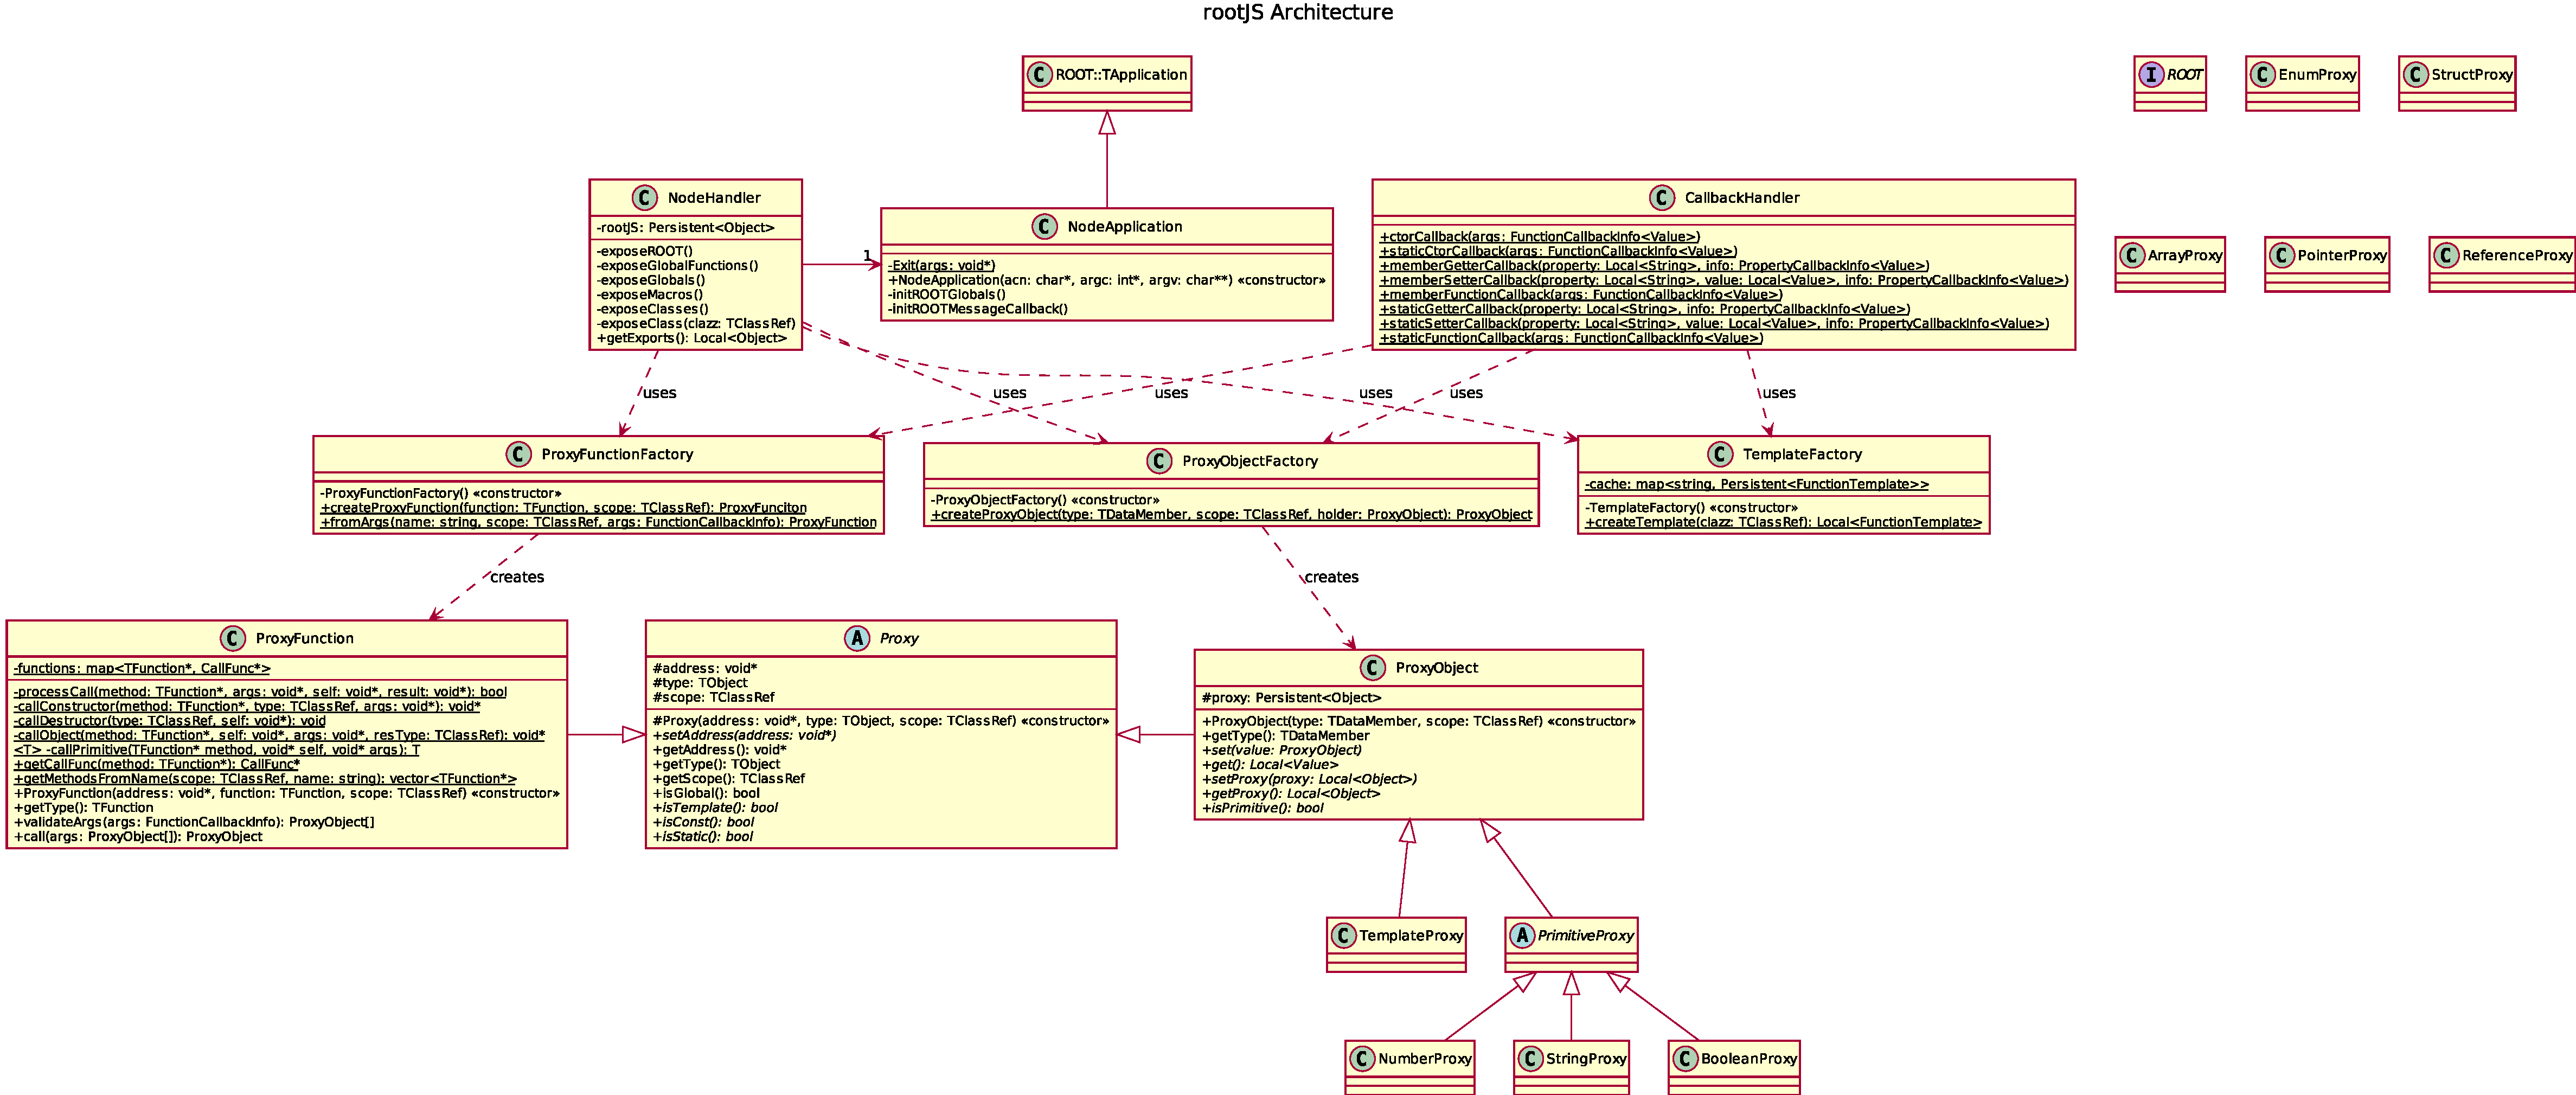
\includegraphics[width=\textheight, height=\linewidth, angle={90}, keepaspectratio]{./latex/resources/architecture.pdf}
	\caption{rootJS class diagram}
\end{figure}

\pagebreak

\section{Dynamic Model}

\begin{figure}[htb]
	\centering
	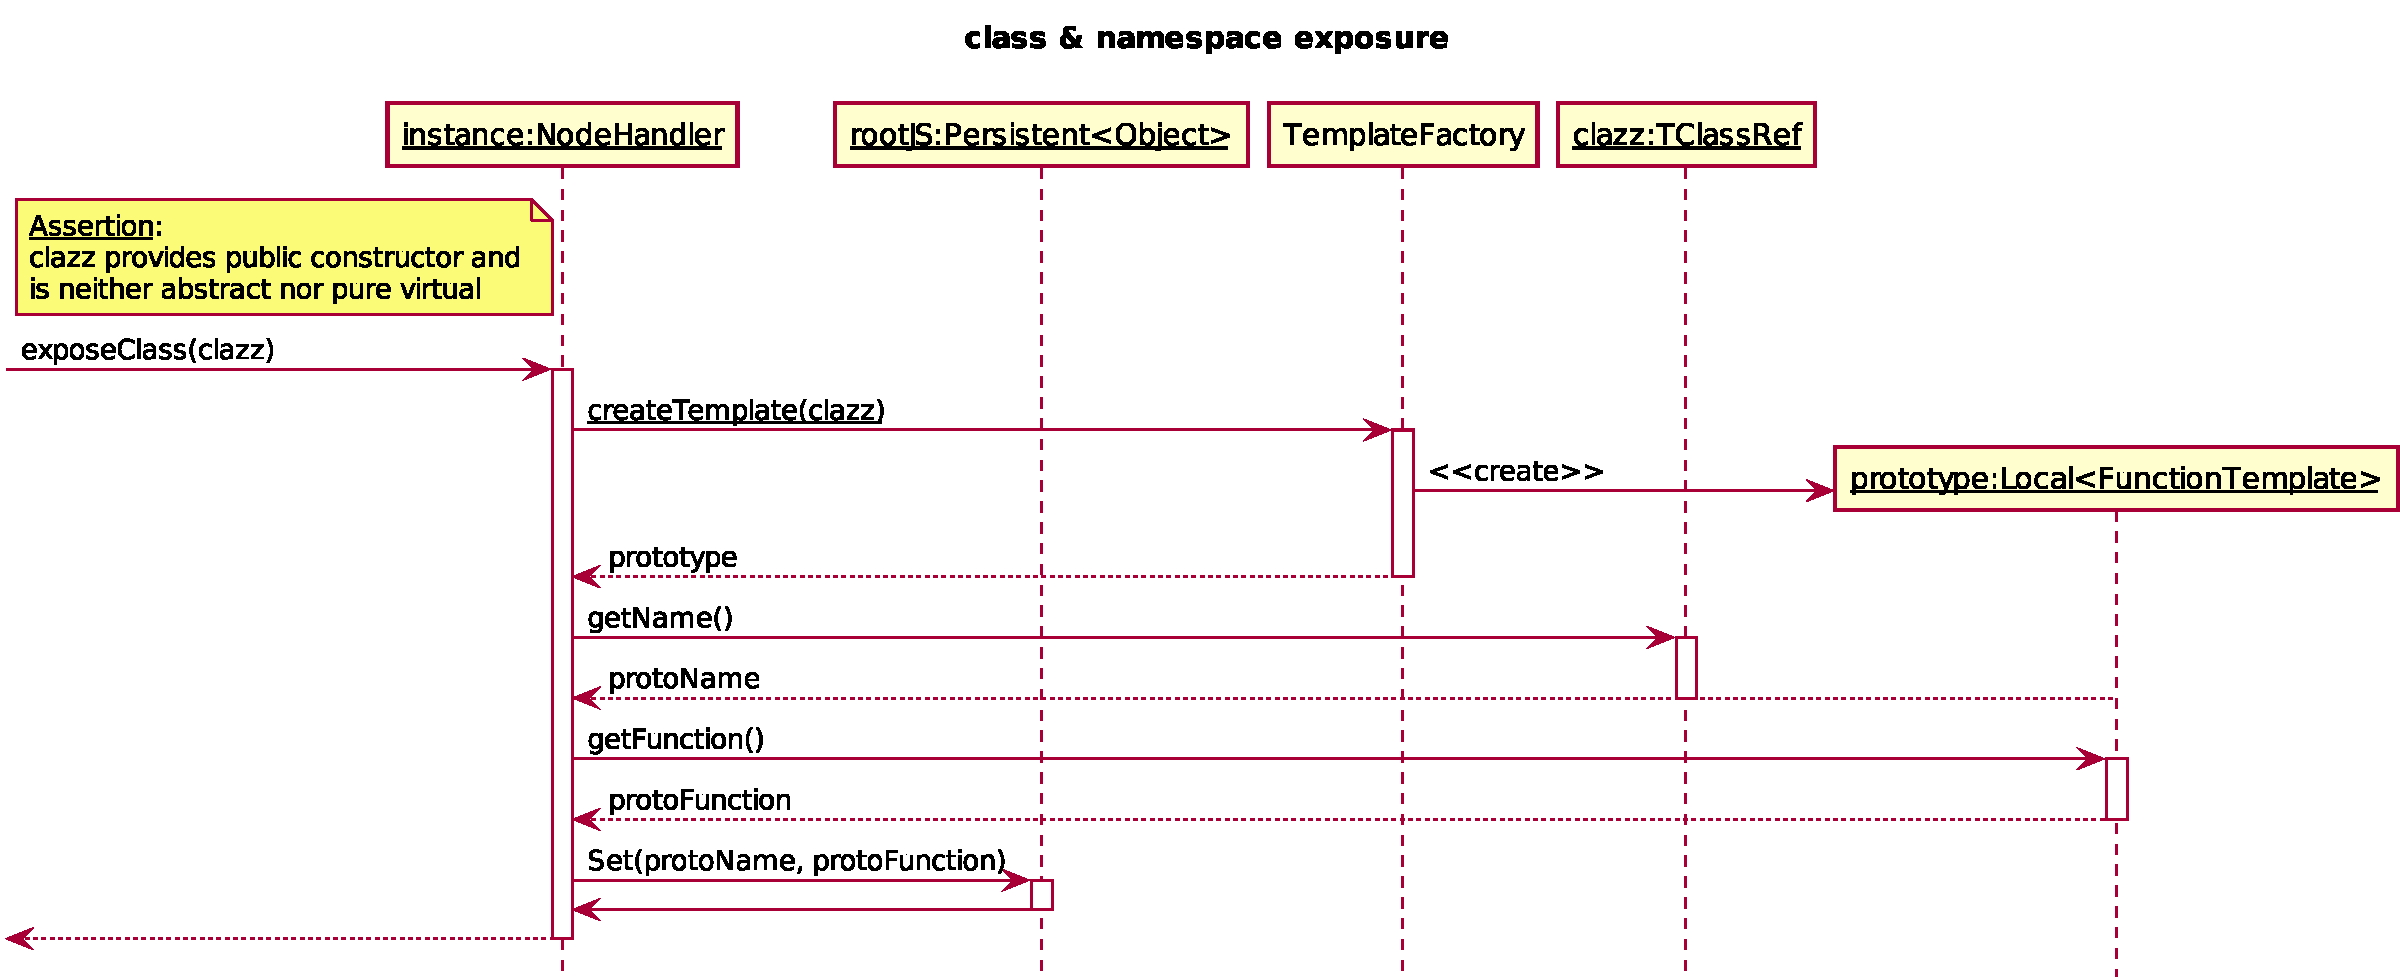
\includegraphics[width=18cm]{./latex/resources/classExposureSequence.pdf}
	\caption{class exposure sequence}
\end{figure}

\begin{figure}[htb]
	\centering
	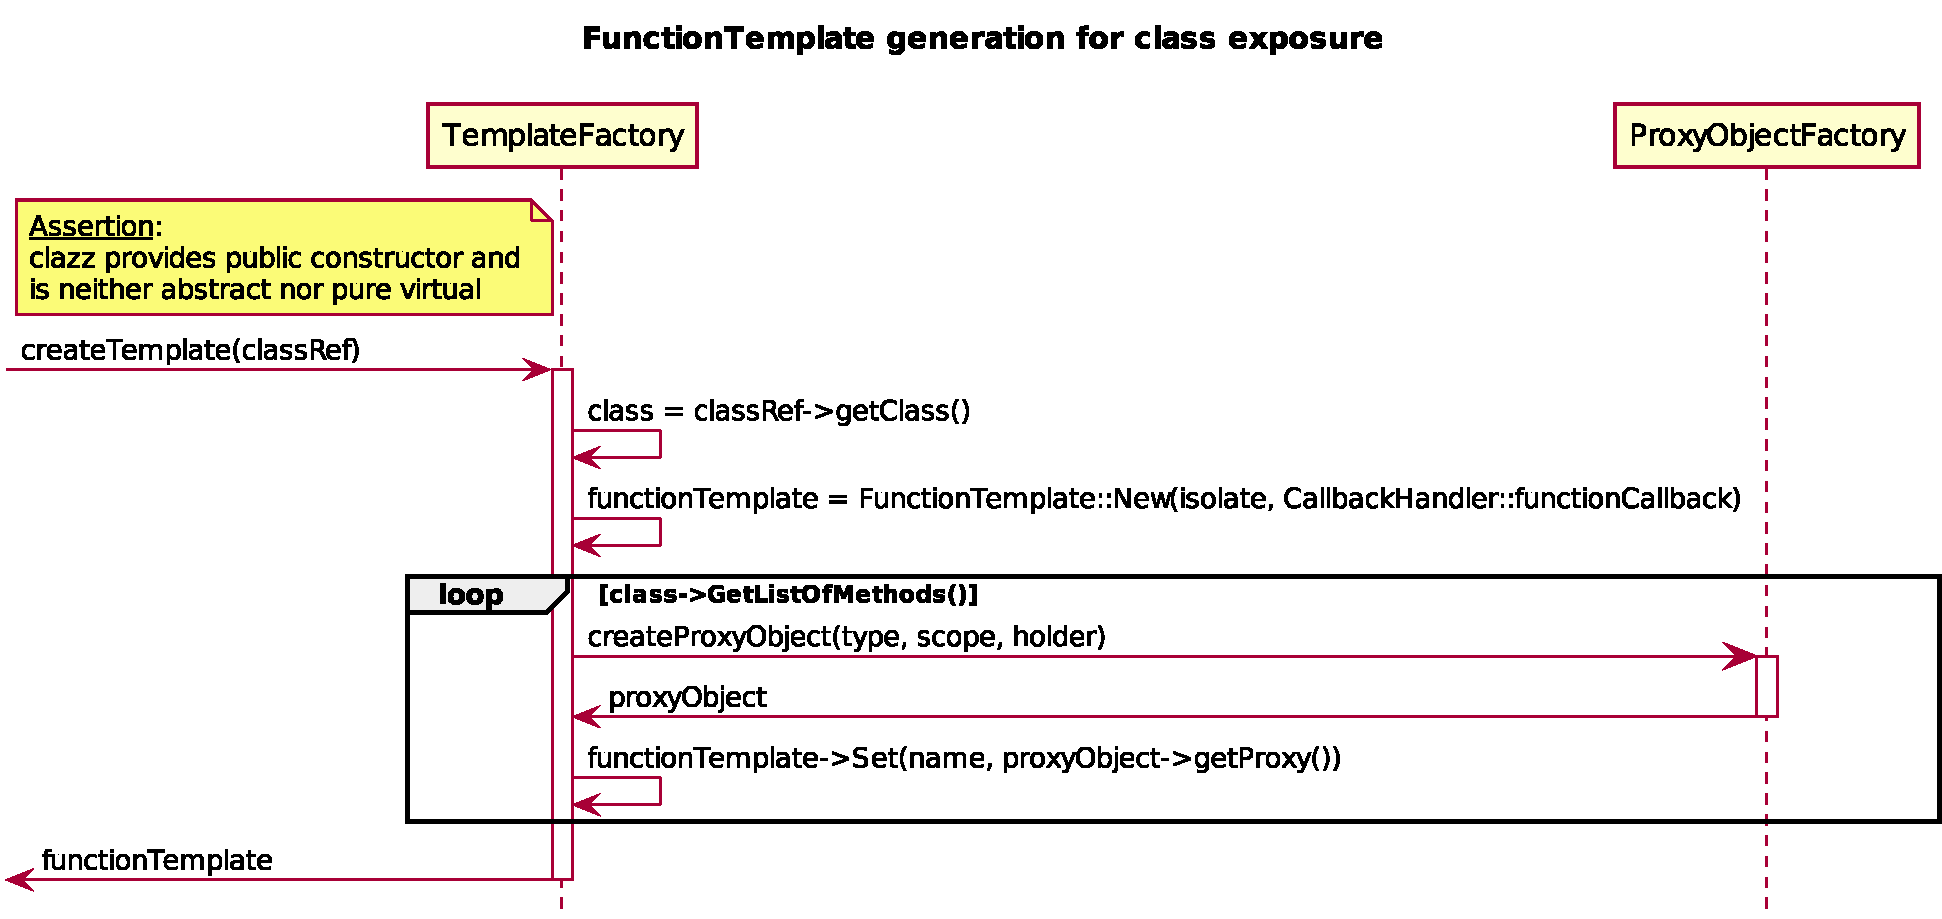
\includegraphics[width=18cm]{./latex/resources/functionTemplateGenerate.pdf}
	\caption{class exposure sequence}
\end{figure}

\begin{figure}[htb]
	\centering
	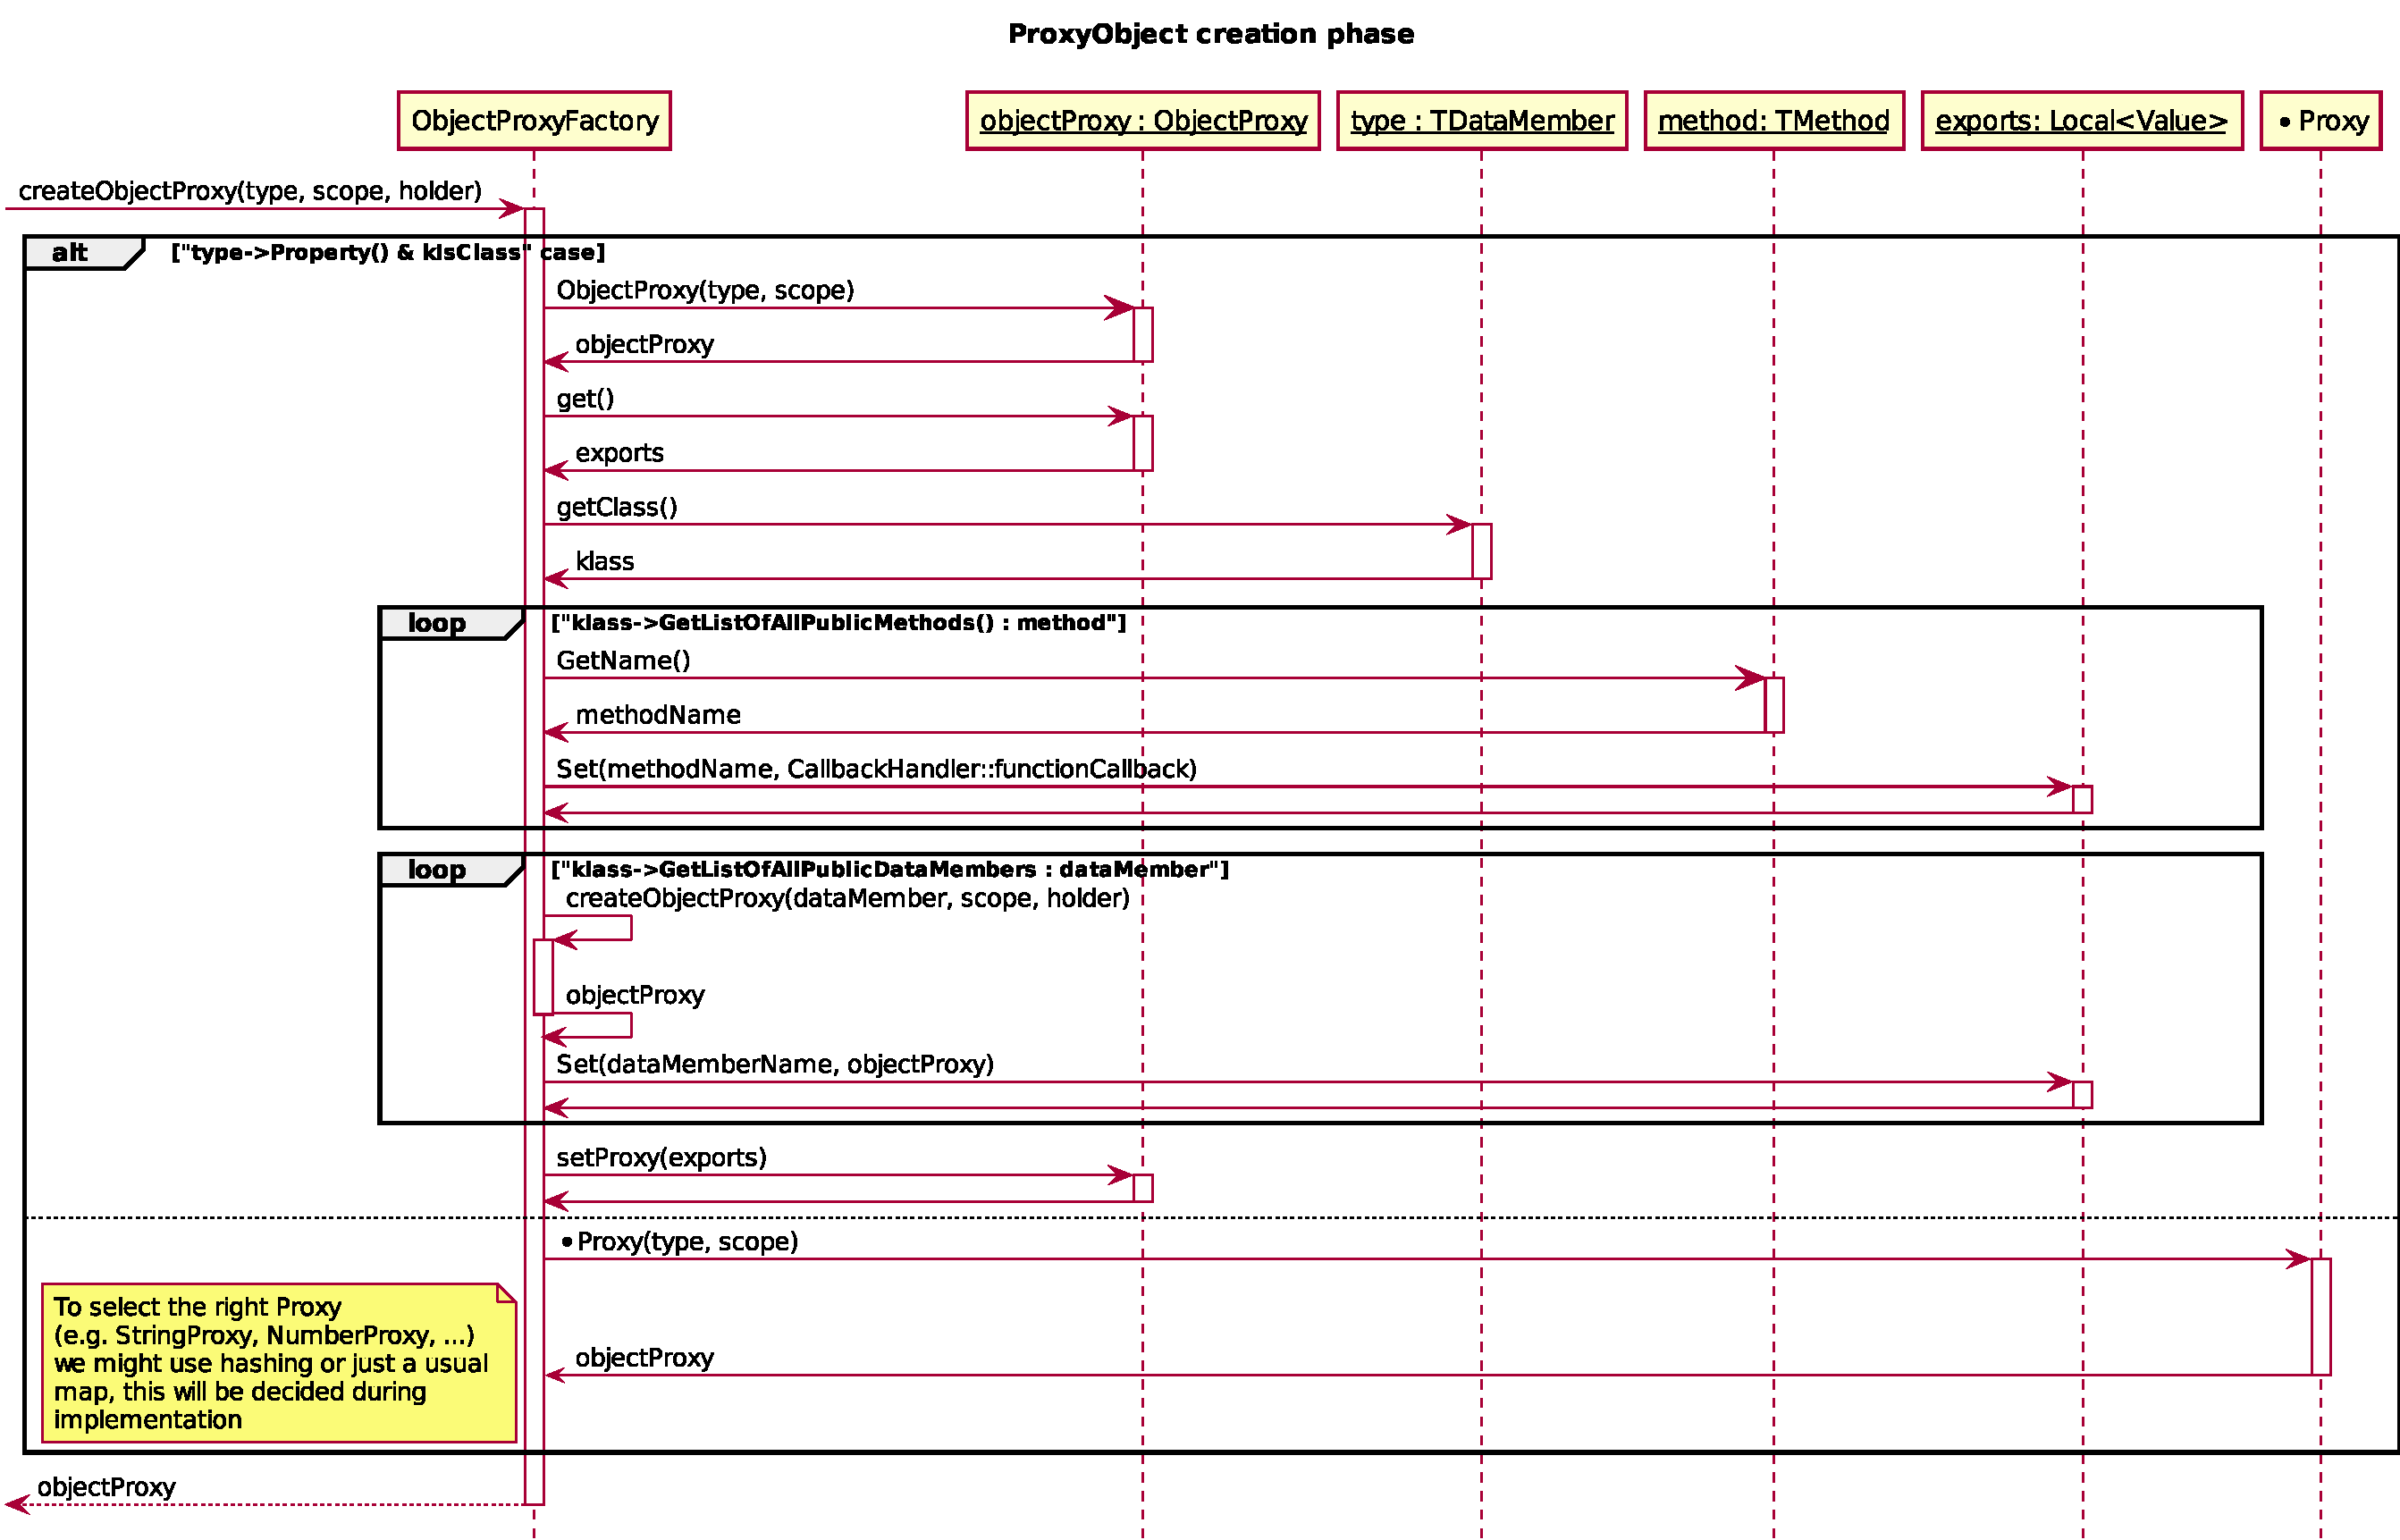
\includegraphics[width=18cm]{./latex/resources/createProxyObject.pdf}
	\caption{ProxyObject creation sequence}
\end{figure}

\newpage

\section{Glossary}
\paragraph{Callback}
A function which is passed as an argument to some code, which is then expected to call the argument back.
\paragraph{Constructor}
A method which is used to create an object.
\paragraph{Encapsulation}
A piece of functionality of certain languages used to restrict access to some of the object's variables and methods
\paragraph{Instance}
A created object.
\paragraph{Proxy}
A class functioning as an intermediary between two classes.
\paragraph{Static}
A method which does not require the object to be instantiated.
\paragraph{Template} 
A feature of C++ that allows classes and functions to operate with generic types.
\paragraph{v8} 
An open source JavaScript engine, written in C++ and made by Google.

\newpage




\end{document}
